\subsubsection{\textit{Câu 3}}

\noindent\textbf{\large Đề bài:} Viết chương trình hợp ngữ cho hai chuỗi ký tự A và B có độ dài là n và m (n > m), chỉ ra xâu B có phải là xâu con của xâu A không? Nếu xâu B là xâu con của xâu A thì chỉ ra vị trí xâu B ở xâu A.

\vspace{0.5cm}
\noindent\textbf{\large Biểu diễn bằng Flowchart:} hình \ref{fig:flowchart-3}

\begin{figure}[H]
    \centering
    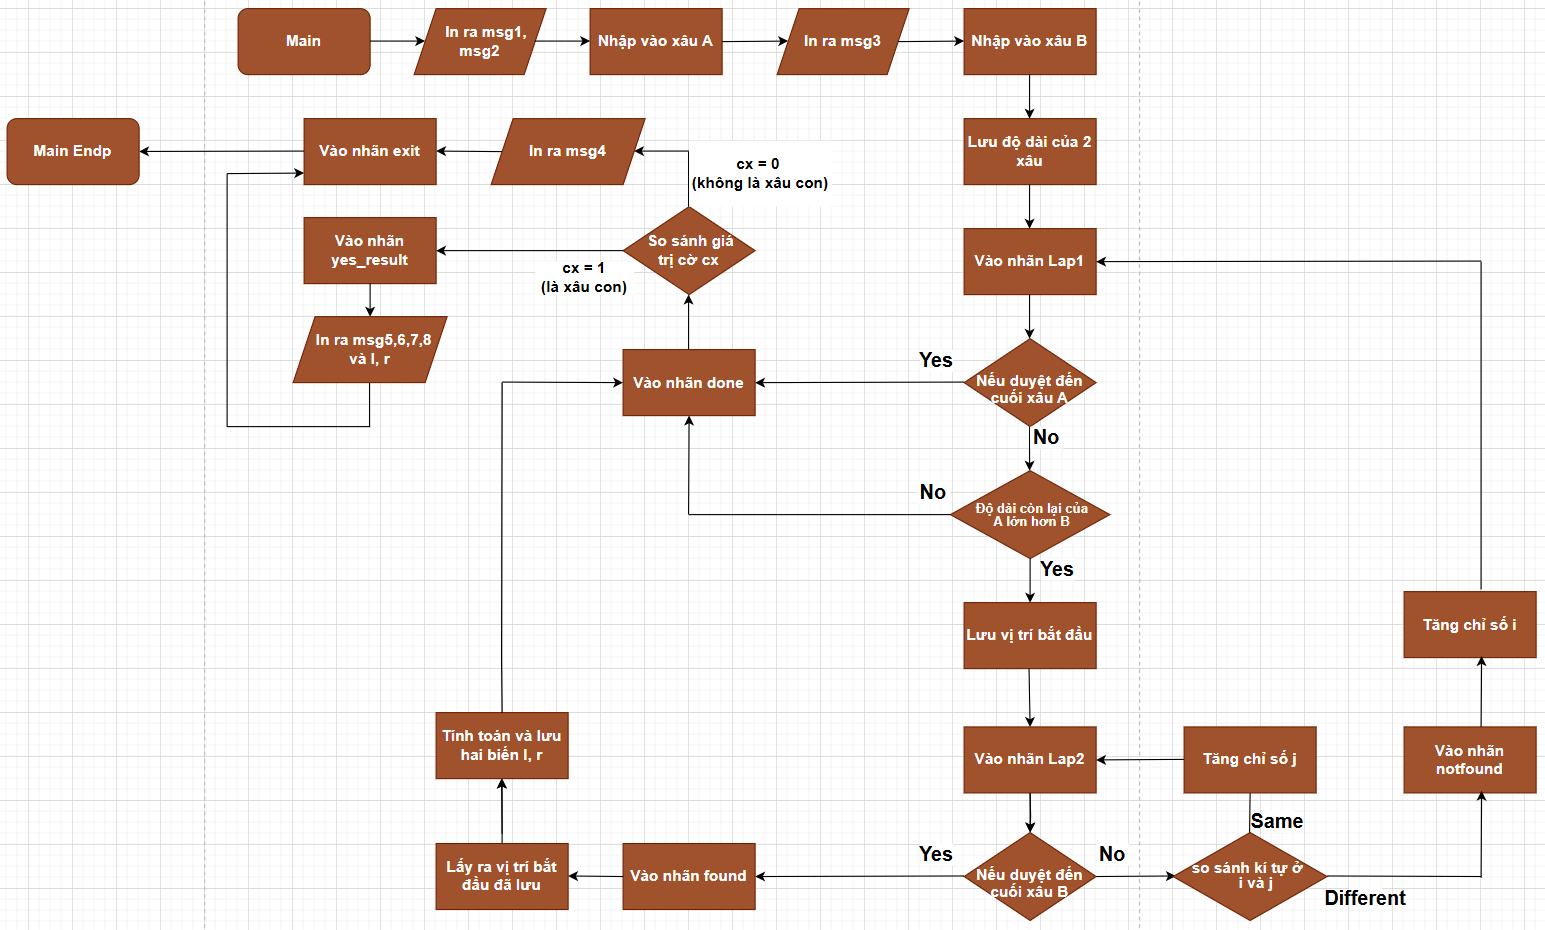
\includegraphics[width=1\textwidth]{Images/Flowchart/Flowchart-3.png}
    \caption{Flowchart kiểm tra xâu con}
    \label{fig:flowchart-3}
\end{figure}

\vspace{0.5cm}
\noindent\textbf{\large Mã nguồn assembly 8086:}
\begin{lstlisting}[style=asm, caption={Mã nguồn câu 3}]
    .model small
    .stack 100
    .data
        crlf db 13, 10, '$'      
        msg1 db 'Nhap vao 2 xau A, B (luu y xau A dai hon xau B)$'
        msg2 db 'Nhap vao xau A: $'
        msg3 db 'Nhap vao xau B: $'
        msg4 db 'B khong la xau con cua A$'      
        msg5 db 'B la xau con cua A$'
        msg6 db 'Vi tri cua B: $'    
        msg7 db 'Tu ki tu $'
        msg8 db ' den ki tu $'
        l dw ?
        r dw ?
        strA db 50, ?, 50 dup('$')
        strB db 50, ?, 50 dup('$')
        lenA db ?
        lenB db ?
    
    .code
    main proc
        mov ax, @data
        mov ds, ax
    
        mov ah, 9                 ;In ra msg1
        lea dx, msg1
        int 21h
        call endl
    
        mov ah, 9                 ;In ra msg2
        lea dx, msg2
        int 21h    
        
        mov ah, 10
        lea dx, strA              ;Nhap xau A
        int 21h
        call endl
    
        mov ah, 9                 ;In ra msg3
        lea dx, msg3
        int 21h      
        
        mov ah, 10                ;Nhap xau B
        lea dx, strB
        int 21h
        call endl
    
        mov al, [strA + 1]        ;Luu do dai strA vao lenA
        mov lenA, al
        mov al, [strB + 1]        ;Luu do dai strB vao lenB
        mov lenB, al                          
        
        lea si, strA + 2           ;si tro vao dau xau A
        mov cx, 0                  ;cx = 0 => chua tim thay
        mov dl, 0                  ;Chi so i trong A
    
        Lap1:
            cmp dl, lenA              ;Neu i >= lenA thi lap xong
            jnl done                   
            mov al, lenA              
            sub al, dl
            cmp al, lenB
            jb done                   ;Phan con lai < do dai B => khong the co xau con
        
            push si                   ;Luu vi tri bat dau
            lea di, strB + 2          ;di tro vao xau B
            mov dh, 0                 ;Chi so j trong B
            mov bx, si                ;bx tro vao vi tri so sanh trong A
        
        Lap2:
            cmp dh, lenB              ;Neu j chay den het strB thi thoa man la xau con
            je found
            mov al, [bx]              ;So sanh chi so i va j
            cmp al, [di]
            jne notfound              ;Neu i != j thi vao nhan not_found
            inc bx                    ;Neu i == j thi tang i, j
            inc di
            inc dh
            jmp Lap2
        
        found:
            pop si                    ;Lay ra vi tri bat dau
            mov cx, 1                 ;cx = 1 => da tim thay
            mov ax, si
            sub ax, offset strA + 2   ;Tinh toan vi tri bat dau
            inc ax                    ;Tang ax vi bat dau tinh tu vi tri 1
            mov l, ax                 ;Luu gia tri vao l
            mov ax, l
            mov bl, lenB              ;Lay vi tri dau tien cong voi
            add ax, bx                ;do dai strB de ra vi tri cuoi cung
            dec ax
            mov r, ax                 ;Luu gia tri vao r
            jmp done
        
        notfound:
            pop si                    ;Neu khong tim thay, tro den vi tri tiep theo trong strA
            inc si
            inc dl
            jmp Lap1
        
        done:
            cmp cx, 1                 ;So sanh cx voi 1 
            je yes_result             ;Neu cx = 1 => vao nhan yes_result
        
            mov ah, 9                 ;Neu cx = 0 => in ra msg4
            lea dx, msg4
            int 21h
            jmp exit
        
        yes_result:
            mov ah, 9                 ;In ra msg5
            lea dx, msg5
            int 21h
            call endl
        
            mov ah, 9                 ;In ra msg6
            lea dx, msg6
            int 21h
        
            mov ah, 9                 ;In ra msg7
            lea dx, msg7
            int 21h
        
            mov ax, l                 ;In ra l
            call InSo
        
            mov ah, 9                 ;In ra msg8
            lea dx, msg8
            int 21h
        
            mov ax, r                 ;In ra r
            call InSo
        
        exit:
        mov ah, 4ch
        int 21h
    main endp
    
    endl proc
        push ax
        push dx
        mov ah, 9
        lea dx, crlf           ;In ra ki tu xuong dong
        int 21h
        pop dx
        pop ax
        ret
    endl endp
    
    InSo proc                       ;Ham in so nguyen
        push ax
        push bx
        push cx
        push dx
    
        mov bx, 10
        mov cx, 0
        next_digit:
            mov dx, 0
            div bx
            push dx
            inc cx
            cmp ax, 0
            jg next_digit
    
        print_digits:
            pop dx
            add dl, '0'
            mov ah, 2
            int 21h
            loop print_digits
    
        pop dx
        pop cx
        pop bx
        pop ax
        ret
    InSo endp
    
    end main
\end{lstlisting}

\vspace{0.5cm}
\noindent\textbf{\large Giao diện hiển thị: } hình \ref{fig:result-3-1} và hình \ref{fig:result-3-2}

\begin{figure}[H]
    \centering
    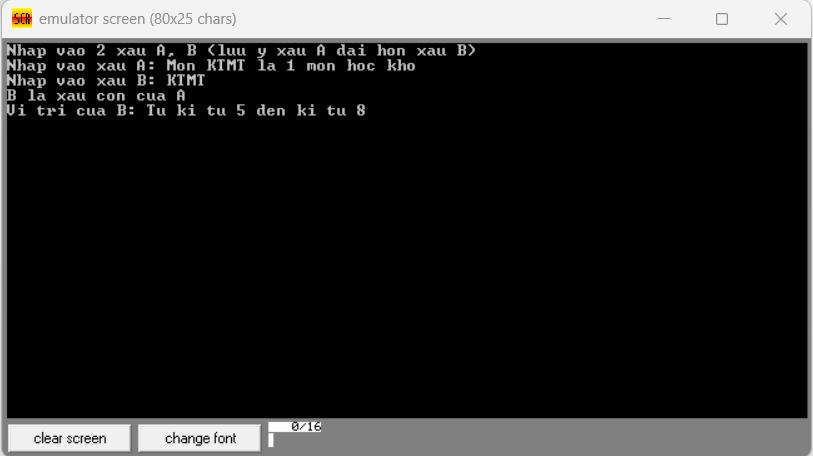
\includegraphics[width=0.8\textwidth]{Images/Result/B3-1.png}
    \caption{Giao diện hiển thị câu 3 - Trường hợp hợp lệ}
    \label{fig:result-3-1}
\end{figure}

\begin{figure}[H]
    \centering
    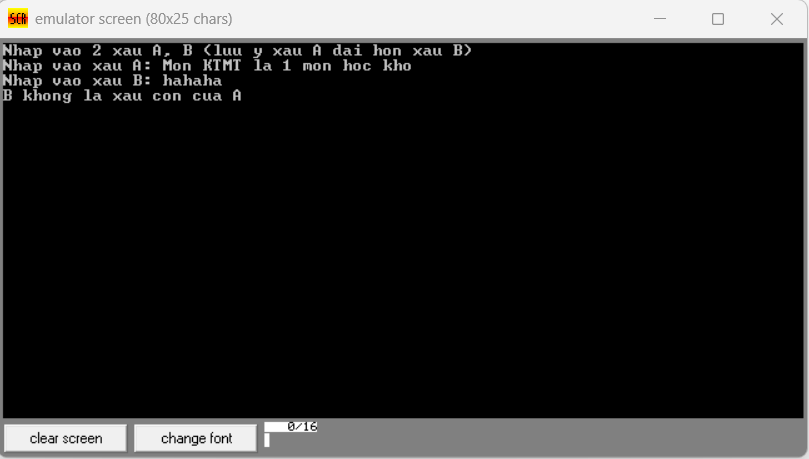
\includegraphics[width=0.8\textwidth]{Images/Result/B3-2.png}
    \caption{Giao diện hiển thị câu 3 - Trường hợp không hợp lệ}
    \label{fig:result-3-2}
\end{figure}

